\section{Metodologie utilizzate}
Per il progetto didattico abbiamo deciso di utilizzare i seguenti approcci: l'algoritmo di \href{https://en.wikipedia.org/wiki/Logistic_regression}{\textit{Logistic Regression}} e le \href{https://en.wikipedia.org/wiki/Neural_network}{\textit{Neural Networks}}.\\
Tuttavia sono possibili altri approcci che, per rimanere all'interno dei tempi stabiliti, non siamo riusciti ad affrontare. 

\subsection{Studio del problema}
Innanzitutto, lo spam è l'invio anche verso indirizzi generici, non verificati o sconosciuti, di messaggi ripetuti ad alta frequenza o a carattere di monotematicità tale da renderli indesiderati. Il problema dello spam nasce quando, con l'avvento di tecnologie informatiche, questa tipologia di messaggi ha iniziato ad invadere le caselle di posta elettronica e gli smartphone di aziende e semplici utilizzatori. Ciò ha portato molte persone ad interessarsi al tema dello spam e di come riuscire a contrastarlo in modo efficace.
\newline
In prima battuta, ci sono state molte discussioni riguardanti la tipologia del problema. Le principali diatribe furono tra chi sosteneva fosse un problema di classificazione e tra chi, invece, sosteneva fosse un problema di modellazione.
Alcune correnti di pensiero continuano a sostenere che la metodologia migliore da applicare in questo caso sia la modellazione, ma la maggior parte della comunità degli studiosi afferma con convinzione che la tecnica migliore sia quella della classificazione. Noi concordiamo con quest'ultimi, vero che il bisogno iniziale di dati già classificati è uno svantaggio, ma nell'era dei big data, è ormai semplice trovare dei set di dati consistenti e pronti all'uso. Inoltre, c'è da sottolineare la maggiore flessibilità della tecnica che è portata maggiormente ad imparare dai propri errori.
\newline
Detto ciò, si può capire perché tra i tanti tipi di approcci al problema abbiamo deciso di utilizzare la Logistic Regression e le Neural Networks, vediamoli ora in modo più approfondito.
\subsection{Reti neurali}
Il primo approccio che abbiamo scelto di utilizzare è stato quello delle reti neurali.
Per farlo ci siamo appoggiati alla libreria \href{https://www.tensorflow.org/}{\textit{TensorFlow}} la quale, dalla versione 2.0.0, integra \href{https://keras.io/}{\textit{Keras}}.\\
Maggiori informazioni riguardanti l'integrazione di Keras sono presenti al seguente link \href{https://www.tensorflow.org/guide/keras}{\textit{tf.keras}}.\\ 
Questo ci ha permesso di:
\begin{enumerate}
\item Utilizzare TensorFlow(\textit{tf}) come ecosistema;
\item Definire la rete tramite la libreria \textit{tf.keras};
\end{enumerate} 
\subsubsection{Struttura}
È stata scelto di utilizzare il tipo di rete \href{https://keras.io/getting-started/sequential-model-guide/}{\textit{Sequential}}.\\ 
Abbiamo creato due reti, con tre layer di tipo \href{https://keras.io/layers/core/}{\textit{Dense}}.
Le funzione di attivazione scelte sono le seguenti:
\begin{enumerate}
\item \href{https://keras.io/activations/#relu}{\textit{Relu}} per i nodi interni;
\item \href{https://keras.io/activations/#sigmoid}{\textit{Sigmoid}} per l'output della rete.
\end{enumerate}
La prima rete presenta la seguente struttura:
\begin{lstlisting}[language=Python]
	model = Sequential()  
	model.add(Dense(512, activation = 'relu')
	model.add(Dense(256, activation = 'relu'))
	model.add(Dense(1, activation = 'sigmoid'))
\end{lstlisting}

La seconda rete presenta la seguente struttura:
\begin{lstlisting}[language=Python]
	model = Sequential()
	model.add(Dense(512, activation = 'relu')
	model.add(Dropout(0.2))
	model.add(Dense(256, activation = 'relu'))
	model.add(Dropout(0.2))
	model.add(Dense(1, activation = 'sigmoid'))
\end{lstlisting}
	 
\subsubsection{Configurazione}
Tramite il metodo \textit{compile()} presente in Keras è possibile stabilire:
\begin{enumerate}
\item \textbf{Loss functions}: \href{https://en.wikipedia.org/wiki/Cross_entropy}{\textit{binary crossentropy}} nel nostro caso, maggiori info al seguente link \href{https://keras.io/losses/}{\textit{loss functions}};
\item \textbf{Optimizer}: l'ottimizzatore che verrà utilizzato per l'aggiustamento dei pesi e per minimizzare la loss function.
Nel nostro caso \href{https://arxiv.org/pdf/1412.6980v8.pdf}{\textit{Adam}}. 
\item \textbf{Metrics}: lista di metriche che verranno valutate dal modello durante la fase di training e testing.
Nel nostro caso è stata scelta la metrica di \href{https://keras.io/metrics/#binary_accuracy}{\textit{binary accuracy}}.  
\end{enumerate} 

\begin{figure}[H]
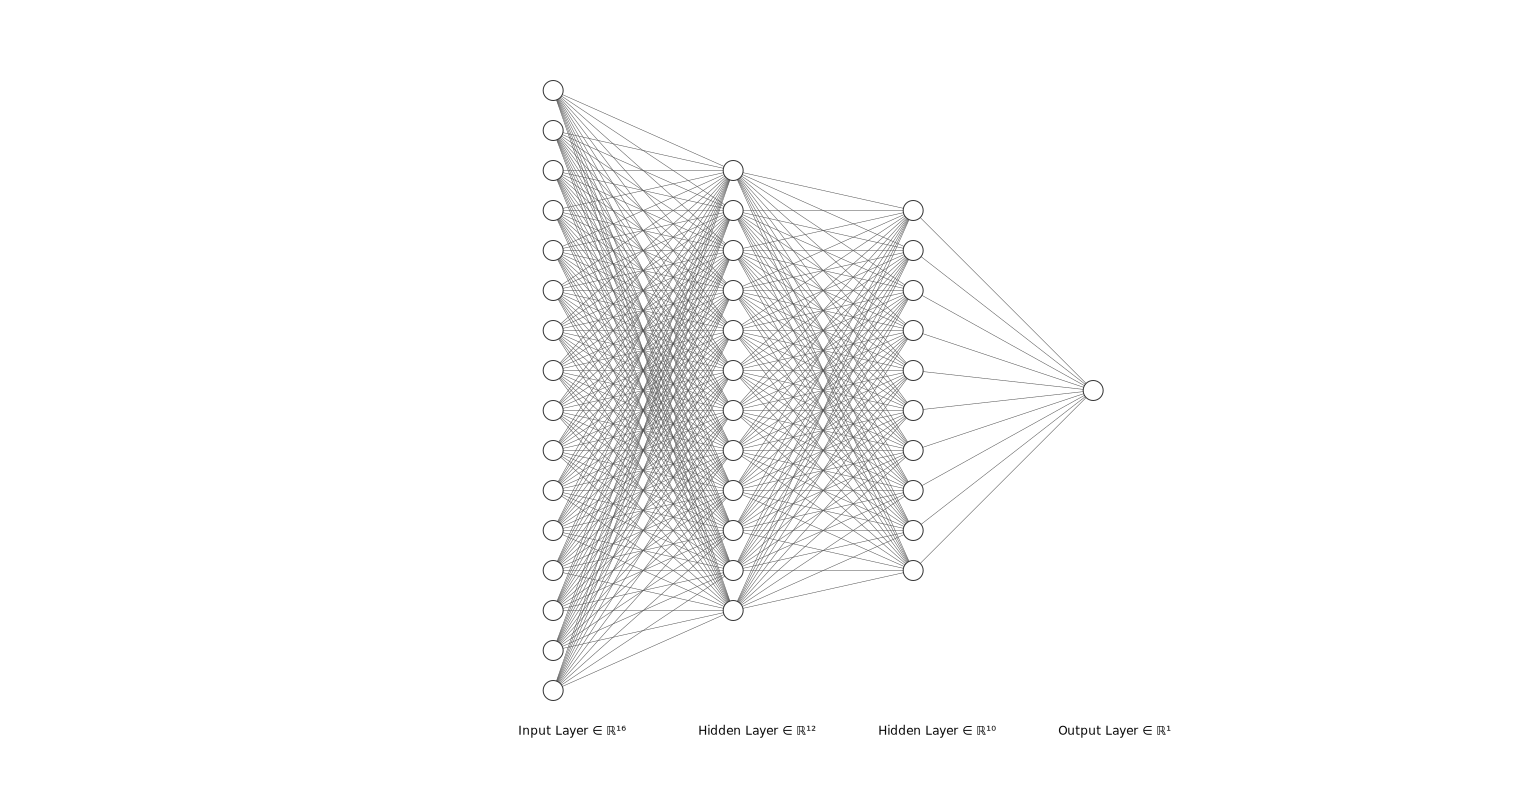
\includegraphics[scale=0.5,center]{img/nnExample.png}
\caption{Esempio di rete neurale}
\end{figure}

Perchè relu, perchè adam, sistema dropout
(TEST SENZA dropout)
\subsection{Logistic Regression}